\documentclass{csc2059practical}

\setmodulecode{CSC2059}
\setmoduletitle{Data Structures and Algorithms}
\setpracticalnumber{1}
\setpracticaltitle{Git Good: Version Control Survival Guide for DSA}
\setpracticalsubtitle{Git, VS Code, branching, merge conflicts, and the CSC2059 workflow}
\setpracticaldate{Academic Year 2026--27}

\usepackage{dirtree}
\usepackage{tabularx}
\usetikzlibrary{positioning,fit,backgrounds}

\newcommand{\checkbox}{\ensuremath{\square}\;}

% Git diff symbols. These can be moved into the template later.
\newcommand{\gitplus}{\textcolor{GitGreen}{\texttt{+}}}
\newcommand{\gitminus}{\textcolor{GitRed}{\texttt{-}}}

\newtcolorbox{terminalplain}{%
  enhanced,
  breakable,
  colback=black!3,
  colframe=black!35,
  boxrule=0.5pt,
  arc=1.5mm,
  left=3mm,right=3mm,top=2mm,bottom=2mm,
  fontupper=\ttfamily\small
}

\newcommand{\CSCModuleWorkflowDiagram}{%
\begin{figure}[H]
\begin{tikzpicture}[
    workflowstep/.style={
        rounded corners,
        draw=CSCBlue,
        fill=CSCBlue!6,
        very thick,
        minimum width=4cm,
        minimum height=1.1cm,
        align=center,
        font=\bfseries
    },
    workflowarrow/.style={
        -{Latex[length=3mm]},
        very thick,
        draw=CSCBlue
    },
    node distance=8mm
]
\node[workflowstep] (edit) {Edit};
\node[workflowstep, below=of edit] (test) {Test};
\node[workflowstep, below=of test] (commit) {Commit};
\node[workflowstep, below=of commit] (push) {Push};
\draw[workflowarrow] (edit) -- (test);
\draw[workflowarrow] (test) -- (commit);
\draw[workflowarrow] (commit) -- (push);
\end{tikzpicture}
\end{figure}}

\newcommand{\CSCGitWorkflowDiagram}{%
\begin{figure}[htbp]
\centering
\begin{tikzpicture}[
  stage/.style={circle, draw=##1!75!black, fill=##1!8, very thick,
    minimum size=21mm, align=center, font=\sffamily\bfseries\scriptsize},
  flow/.style={-{Latex[length=3mm]}, very thick, draw=CSCBlue!70},
  captionnote/.style={font=\sffamily\small, align=center, text=black!80}
]
\node[stage=CSCBlue] (edit) at (90:28mm) {Edit};
\node[stage=CSCAmber] (test) at (18:28mm) {Test};
\node[stage=CSCGreen] (commit) at (-54:28mm) {Commit};
\node[stage=CSCPurple] (push) at (-126:28mm) {Push};
\node[stage=CSCBlue] (repeat) at (162:28mm) {Repeat};
\draw[flow] (edit) -- (test);
\draw[flow] (test) -- (commit);
\draw[flow] (commit) -- (push);
\draw[flow] (push) -- (repeat);
\draw[flow] (repeat) -- (edit);
\node[captionnote] at (0,0) {small steps};
\end{tikzpicture}
\caption{The basic CSC2059 Git workflow.}
\end{figure}%
}

\newcommand{\CSCGitAreasDiagram}{%
\begin{figure}[htbp]
\centering
\begin{tikzpicture}[
  box/.style={draw=CSCBlue!70!black, fill=CSCBlue!6, rounded corners=2mm, very thick,
    minimum width=40mm, minimum height=16mm, align=center, font=\sffamily\small\bfseries},
  arrow/.style={-{Latex[length=3mm]}, very thick, draw=CSCBlue!75!black},
  lab/.style={font=\sffamily\scriptsize, align=center, text=black!75}
]
\node[box] (work) {Working area\\\footnotesize files you edit};
\node[box, right=18mm of work] (stage) {Staging area\\\footnotesize changes selected};
\node[box, right=18mm of stage] (hist) {Commit history\\\footnotesize saved snapshots};
\draw[arrow] (work) -- node[above,lab]{\texttt{git add}} (stage);
\draw[arrow] (stage) -- node[above,lab]{\texttt{git commit}} (hist);
\end{tikzpicture}
\caption{The three places your work can exist in a local Git repository.}
\end{figure}%
}

\newcommand{\CSCGitBranchSplitDiagram}{%
\begin{figure}[htbp]
\centering
\begin{tikzpicture}[
  commit/.style={circle, draw=CSCBlue!70!black, fill=CSCBlue!8, very thick, minimum size=8mm, font=\sffamily\bfseries\scriptsize},
  feature/.style={circle, draw=CSCPurple!70!black, fill=CSCPurple!8, very thick, minimum size=8mm, font=\sffamily\bfseries\scriptsize},
  line/.style={very thick, draw=black!55},
  label/.style={font=\sffamily\small, align=center}
]
\node[commit] (A) at (0,0) {A};
\node[commit] (B) at (1.6,0) {B};
\node[commit] (C) at (3.2,0) {C};
\node[feature] (D) at (4.8,-1.2) {D};
\draw[line] (A) -- (B) -- (C);
\draw[line] (C) -- (D);
\node[label, above=3mm of A] {main};
\node[label, right=4mm of D] {feature-message\\\scriptsize Improve message};
\node[label, below=14mm of C, text width=75mm] {The feature branch has one commit that does not yet exist on \texttt{main}.};
\end{tikzpicture}
\caption{A feature branch created from \texttt{main}.}
\end{figure}%
}

\newcommand{\CSCGitFastForwardDiagram}{%
\begin{figure}[htbp]
\centering
\begin{tikzpicture}[
  commit/.style={circle, draw=CSCGreen!70!black, fill=CSCGreen!8, very thick, minimum size=8mm, font=\sffamily\bfseries\scriptsize},
  line/.style={very thick, draw=black!55},
  label/.style={font=\sffamily\small, align=center}
]
\node[commit] (A) at (0,0) {A};
\node[commit] (B) at (1.6,0) {B};
\node[commit] (C) at (3.2,0) {C};
\node[commit] (D) at (4.8,0) {D};
\draw[line] (A) -- (B) -- (C) -- (D);
\node[label, above=3mm of D] {main, feature-message};
\node[label, below=6mm of C, text width=80mm] {After a fast-forward merge, \texttt{main} simply moves forward to include commit D.};
\end{tikzpicture}
\caption{The branch after a successful fast-forward merge.}
\end{figure}%
}

\newcommand{\CSCGitConflictDiagram}{%
\begin{figure}[htbp]
\centering
\begin{tikzpicture}[
  commit/.style={circle, draw=CSCBlue!70!black, fill=CSCBlue!8, very thick, minimum size=8mm, font=\sffamily\bfseries\scriptsize},
  maincommit/.style={circle, draw=CSCAmber!75!black, fill=CSCAmber!12, very thick, minimum size=8mm, font=\sffamily\bfseries\scriptsize},
  featurecommit/.style={circle, draw=CSCPurple!75!black, fill=CSCPurple!10, very thick, minimum size=8mm, font=\sffamily\bfseries\scriptsize},
  line/.style={very thick, draw=black!55},
  label/.style={font=\sffamily\small, align=center}
]
\node[commit] (A) at (0,0) {A};
\node[commit] (B) at (1.4,0) {B};
\node[commit] (C) at (2.8,0) {C};
\node[commit] (D) at (4.2,0) {D};
\node[maincommit] (F) at (5.9,0.9) {F};
\node[featurecommit] (E) at (5.9,-0.9) {E};
\draw[line] (A) -- (B) -- (C) -- (D);
\draw[line] (D) -- (F);
\draw[line] (D) -- (E);
\node[label, right=4mm of F] {main\\\scriptsize confusion};
\node[label, right=4mm of E] {feature-warning\\\scriptsize panic};
\node[label, below=9mm of D, text width=82mm] {Both branches changed the same line in different ways, so Git cannot safely choose for you.};
\end{tikzpicture}
\caption{Two branches making conflicting changes to the same line.}
\end{figure}%
}

\newcommand{\CSCGitConflictResolvedDiagram}{%
\begin{figure}[htbp]
\centering
\begin{tikzpicture}[
  commit/.style={circle, draw=CSCBlue!70!black, fill=CSCBlue!8, very thick, minimum size=8mm, font=\sffamily\bfseries\scriptsize},
  maincommit/.style={circle, draw=CSCAmber!75!black, fill=CSCAmber!12, very thick, minimum size=8mm, font=\sffamily\bfseries\scriptsize},
  featurecommit/.style={circle, draw=CSCPurple!75!black, fill=CSCPurple!10, very thick, minimum size=8mm, font=\sffamily\bfseries\scriptsize},
  mergecommit/.style={circle, draw=CSCGreen!75!black, fill=CSCGreen!10, very thick, minimum size=8mm, font=\sffamily\bfseries\scriptsize},
  line/.style={very thick, draw=black!55},
  label/.style={font=\sffamily\small, align=center}
]
\node[commit] (A) at (0,0) {A};
\node[commit] (B) at (1.4,0) {B};
\node[commit] (C) at (2.8,0) {C};
\node[commit] (D) at (4.2,0) {D};
\node[maincommit] (F) at (5.8,0.9) {F};
\node[featurecommit] (E) at (5.8,-0.9) {E};
\node[mergecommit] (G) at (7.5,0) {G};
\draw[line] (A) -- (B) -- (C) -- (D);
\draw[line] (D) -- (F) -- (G);
\draw[line] (D) -- (E) -- (G);
\node[label, right=4mm of G] {resolved merge\\\scriptsize both ideas combined};
\node[label, below=9mm of D, text width=90mm] {After you resolve the conflict, Git records a new merge commit.};
\end{tikzpicture}
\caption{The conflict resolved with a merge commit.}
\end{figure}%
}

\newcommand{\CSCGitRemoteDiagram}{%
\begin{figure}[htbp]
\centering
\begin{tikzpicture}[
  box/.style={draw=CSCPurple!70!black, fill=CSCPurple!6, rounded corners=2mm, very thick,
    minimum width=40mm, minimum height=16mm, align=center, font=\sffamily\small\bfseries},
  arrow/.style={-{Latex[length=3mm]}, very thick, draw=CSCPurple!75!black},
  lab/.style={font=\sffamily\scriptsize, align=center, text=black!75}
]
\node[box] (local) {Local repository\\\footnotesize on your computer};
\node[box, right=26mm of local] (remote) {Remote repository\\\footnotesize on GitHub/Classroom50};
\draw[arrow] (local) -- node[above,lab]{\texttt{git push}} (remote);
\draw[arrow] (remote) to[bend left=18] node[below,lab]{\texttt{git clone} / \texttt{git pull}} (local);
\end{tikzpicture}
\caption{Commits must be pushed before they exist in the remote repository.}
\end{figure}%
}

\begin{document}
\maketitle
\tableofcontents
\clearpage
\frontsection{Welcome}
Welcome to the first lab of CSC2059 Data Structures and Algorithms. Over the coming weeks, you will learn how to design and implement data structures, analyse algorithms, solve computational problems, and write increasingly sophisticated C++ programs.

Before we start building stacks, queues, linked lists, trees, and algorithms, we need one essential tool used by professional software developers: version control.

That tool is \textbf{Git}.

Git allows you to keep track of changes, recover from mistakes, collaborate safely with others, and submit work through Classroom50. It is one of the most widely used tools in software development and will be used throughout this module.

More importantly, Git can save you from many of the most common student disasters:

\begin{itemize}
  \item Accidentally overwriting your work.
  \item Deleting code that was working five minutes ago.
  \item Losing track of which version is the latest.
  \item Realising after an assessment that your work was never submitted.
\end{itemize}
Don't worry if you've never used Git before. By the end of this lab, you will have created repositories, made commits, worked with branches, resolved a merge conflict, and submitted code to an online repository using the same workflow that will be used throughout CSC2059.

\frontsection{Learning Objectives}
\begin{learningoutcomes}
By the end of this lab, you should be able to:

\begin{enumerate}
  \item Configure Git for personal use on a local machine.
  \item Create and manage a local Git repository.
  \item Stage, commit, and inspect changes using Git.
  \item Use Git through both the command line and Visual Studio Code.
  \item Create, merge, and manage branches.
  \item Resolve a simple merge conflict.
  \item Clone, modify, commit, and push changes to a remote repository.
  \item Follow a professional software development workflow when working on C++ programs.
\end{enumerate}
\end{learningoutcomes}
\paragraph{In Plain English...}
By the end of this lab, you should be able to:

\begin{itemize}
  \item \faCheck\ Configure Git without needing emergency technical support.
  \item \faCheck\ Save your work properly instead of creating files called:
\end{itemize}
\begin{terminalplain}
assignment.cpp

assignment\_final.cpp

assignment\_final\_v2.cpp

assignment\_final\_v2\_REALLY\_FINAL.cpp

assignment\_final\_v2\_REALLY\_FINAL\_FIXED.cpp
\end{terminalplain}
\begin{itemize}
  \item \faCheck\ Understand what Git is trying to tell you when it displays alarming-looking messages.
  \item \faCheck\ Survive your first merge conflict without questioning your career choices.
  \item \faCheck\ Use the same workflow that will be used throughout CSC2059.
\end{itemize}
Most importantly:

\begin{itemize}
  \item \faCheck\ Avoid discovering ten minutes before a class test ends that your code was never committed and never pushed.
\end{itemize}
\subsection*{Git in 30 Seconds}
Think of Git as a save-game system for programmers.

When writing code, you typically:

\begin{enumerate}
  \item Make some changes.
  \item Decide which changes you want to keep.
  \item Create a snapshot of those changes (called a commit).
  \item Upload that snapshot to a remote repository.
\end{enumerate}
Git keeps a history of these snapshots so that progress can be tracked and mistakes can often be undone.

You do not need to understand all the internal details of Git to use it successfully. In this lab, we will focus on the practical skills that you will use every week throughout the module.

\clearpage
\frontsection{The CSC2059 Workflow}
\begin{workflowreminder}
Throughout this module, we will repeatedly follow the same workflow:

\CSCModuleWorkflowDiagram

Where:

\begin{itemize}
  \item \textbf{Edit} means changing your code.
  \item \textbf{Test} means checking that it works.
  \item \textbf{Commit} means creating a snapshot of your progress.
  \item \textbf{Push} means sending that snapshot to the online repository.
\end{itemize}
If you remember only one thing from today's lab, remember this workflow.

\end{workflowreminder}
\frontsection{How This Lab Works}
This lab is designed to be completed by doing, not by reading.

You will:

\begin{itemize}
  \item Create your own Git repository.
  \item Make changes and commit them.
  \item Use Git from both the command line and Visual Studio Code.
  \item Create and merge branches.
  \item Resolve a merge conflict.
\end{itemize}
Along the way, you will make mistakes.

This is expected.

In fact, some of the mistakes in this lab are intentional.

It is far better to learn how to recover from a problem in Week 1 than during an assessment.

Let's get started.

\section{Preparing Your Development Environment}
\begin{infobox}
\textbf{Estimated time: 5 minutes}
\end{infobox}

The software required for CSC2059 must be installed before you begin the practical exercises. This practical does not reproduce the installation instructions.

\subsection{Using Your Own Windows Computer}

If you are working on your own Windows laptop or PC, follow the separate \textbf{CSC2059 Development Environment: Windows Installation Guide} before continuing with this practical.

That guide installs and configures Visual Studio Code, Git, MSYS2 and the C++ development tools used throughout CSC2059. It also configures \textbf{CSC2059 Terminal} as the default terminal profile in Visual Studio Code.

Once the installation guide has been completed, selecting:

\begin{terminalplain}
Terminal -> New Terminal
\end{terminalplain}

should normally open the CSC2059 Terminal automatically.

\subsection{Using a University Laboratory Computer}

The required software is already installed on the School laboratory computers. However, the default Visual Studio Code terminal on the laboratory machines is PowerShell.

For CSC2059 work, Windows users should use the \textbf{CSC2059 Terminal} instead.

Open Visual Studio Code and select:

\begin{terminalplain}
Terminal -> New Terminal
\end{terminalplain}

If PowerShell opens, use the terminal profile selector in the terminal panel and choose:

\begin{terminalplain}
CSC2059 Terminal
\end{terminalplain}

\clearpage

\begin{importantnote}
\textbf{Windows Users}\par
\medskip

Use the \textbf{CSC2059 Terminal} for CSC2059 practical work.

Do not use PowerShell, Command Prompt, or Git Bash for the command-line activities in this module.
\end{importantnote}

\subsection{macOS and Linux}

On macOS or Linux, use the integrated terminal in Visual Studio Code. No special CSC2059 terminal profile is required.

\subsection{Verify the Development Environment}

Before continuing, Windows users should confirm that the correct CSC2059 environment is active.

Run:

\begin{terminalplain}
which g++

which make

which git
\end{terminalplain}

On the School Windows laboratory machines, and on a Windows computer configured using the CSC2059 installation guide, the expected paths are:

\begin{terminalplain}
/ucrt64/bin/g++

/usr/bin/make

/usr/bin/git
\end{terminalplain}

All users should also check that Git is available:

\begin{terminalplain}
git \mintinline{text}{--version}
\end{terminalplain}

You should see a Git version number. The exact version may differ between computers.

\begin{reflectionbox}
\textbf{Checkpoint}\par
\medskip

Before continuing, confirm that Visual Studio Code is running correctly and that Git is available from the terminal.

Windows users should also confirm that \textbf{CSC2059 Terminal} is the active terminal profile and that the three paths above are reported correctly.
\end{reflectionbox}

\begin{wrapupbox}
\textbf{Environment Ready}\par
\medskip

You now have the development environment needed for this practical.

In the next section, you will configure Git so that your commits are correctly attributed to you.
\end{wrapupbox}

\section{Configuring Git}
\begin{infobox}
\textbf{Estimated time: 5-10 minutes}
\end{infobox}
Now that the development environment is ready, we need to tell Git who you are.

Every commit created with Git records information about its author. This allows you, your teammates, and your lecturers to see who made a particular change and when it was made.

Before you start using Git, you should configure your name and email address.

\begin{learningoutcomes}
\textbf{What You Will Learn}\par
\medskip
By the end of this section, you should be able to:

\begin{itemize}
  \item Configure your Git username.
  \item Configure your Git email address.
  \item View your current Git configuration.
  \item Understand the difference between global and repository-specific settings.
\end{itemize}
\end{learningoutcomes}
\begin{importantnote}
Throughout this module, we recommend using your university email address when configuring Git.

This will make it easier for services such as GitHub and Classroom50 to associate your work with your account.
\end{importantnote}

Open Visual Studio Code.

Open a new terminal:

Terminal → New Terminal

\begin{importantnote}
\textbf{Windows Lab Computers}\par
\medskip

If the terminal opens as PowerShell, use the terminal profile selector and choose \textbf{CSC2059 Terminal} before entering the commands below.
\end{importantnote}

You should now be ready to enter Git commands.

\subsection{Global Configuration}
Global settings apply to \textbf{all Git repositories on the current computer}.

For most users, this is the simplest option.

\subsubsection{Step 1: Configure Your Name}
Replace the example name below with your own name.

\begin{terminalplain}
git config \mintinline{text}{--global} user.name "Bruce Wayne"
\end{terminalplain}
For example:

\begin{terminalplain}
git config \mintinline{text}{--global} user.name "Jane Smith"
\end{terminalplain}
Press \textbf{Enter}.

If the command completes successfully, Git will not display any output.

This is normal.

\subsubsection{Step 2: Configure Your Email Address}
Replace the example email address below with your own university email address.

\begin{terminalplain}
git config \mintinline{text}{--global} user.email "batman@batcave.com"
\end{terminalplain}
For example:

\begin{terminalplain}
git config \mintinline{text}{--global} user.email "jsmith123@qub.ac.uk"
\end{terminalplain}
Press \textbf{Enter}.

Again, Git will normally display no output.

This is normal.

\subsubsection{Step 3: Verify Your Configuration}
Run:

\begin{terminalplain}
git config \mintinline{text}{--list}
\end{terminalplain}
You should see output containing lines similar to:

\begin{terminalplain}
user.name=Jane Smith
\end{terminalplain}
\begin{terminalplain}
user.email=jsmith123@qub.ac.uk
\end{terminalplain}
You may see additional settings as well.

That is perfectly normal.

\begin{reflectionbox}
\textbf{Checkpoint}\par
\medskip
Before continuing, confirm that:
\end{reflectionbox}
\begin{terminalplain}
git config \mintinline{text}{--list} runs successfully.
\end{terminalplain}
Your name appears in the output.

Your email address appears in the output.

If all three boxes are checked, your global Git configuration is working correctly.

\subsection{Repository-Specific Configuration}
Sometimes you may want to configure Git for a single repository rather than for the entire computer.

This is known as a \textbf{local configuration}.

For example:

\begin{terminalplain}
git config user.name "Jane Smith"
\end{terminalplain}
\begin{terminalplain}
git config user.email "1234567@qub.ac.uk"
\end{terminalplain}
Notice that the \mintinline{text}{--global} option is missing.

These settings apply only to the current repository.

\begin{importantnote}
  \textbf{Why Would I Use This?}

  Most of the time, you will not need to.
  
  However, there is one situation where local configuration can be useful.
  
  The laboratory machines are periodically reset.
  
  This means that global settings may disappear between sessions.
  
  If necessary, you can configure a repository individually using the commands above.
  
  For now, simply be aware that this option exists.
\end{importantnote}

\subsection{Common Problems}
\begin{commonerror}
\textbf{I Ran the Command and Nothing Happened}\par
\medskip
Good.

Many Git commands complete successfully without displaying any output.

Run:
\begin{terminalplain}
  git config \mintinline{text}{--list}
\end{terminalplain}
to verify that the settings were applied.
\end{commonerror}

\begin{commonerror}
\textbf{My Name or Email Is Incorrect}\par
\medskip
Simply run the command again with the correct information.

For example:
\begin{terminalplain}
  git config \mintinline{text}{--global} user.name "Correct Name"
\end{terminalplain}
\begin{terminalplain}
  git config \mintinline{text}{--global} user.email "correct.email@example.com"
\end{terminalplain}
The old values will be replaced automatically.
\end{commonerror}

\begin{commonerror}
\textbf{I Can't Remember My Current Settings}\par
\medskip
Run:
\begin{terminalplain}
  git config \mintinline{text}{--list}
\end{terminalplain}
This will display your current Git configuration.
\end{commonerror}

\subsection{Quick Reference}
Display current configuration:

\begin{terminalplain}
git config \mintinline{text}{--list}
\end{terminalplain}
Set global username:

\begin{terminalplain}
git config \mintinline{text}{--global} user.name "Your Name"
\end{terminalplain}
Set global email:

\begin{terminalplain}
git config \mintinline{text}{--global} user.email "your.email@example.com"
\end{terminalplain}
Set repository-specific username:

\begin{terminalplain}
git config user.name "Your Name"
\end{terminalplain}
Set repository-specific email:

\begin{terminalplain}
git config user.email "your.email@example.com"
\end{terminalplain}
\begin{importantnote}
\textbf{Remember This}\par
\medskip
If Git ever complains that it does not know who you are, or refuses to create a commit because your identity is unknown, return to this section and run:

\begin{terminalplain}
  git config \mintinline{text}{--list}
\end{terminalplain}
to check your current settings.

If your name or email address is missing, re-run the configuration commands:

\begin{terminalplain}
  git config \mintinline{text}{--global} user.name "Your Name"
\end{terminalplain}
\begin{terminalplain}
  git config \mintinline{text}{--global} user.email "your.email@example.com"
\end{terminalplain}
This situation is particularly common on laboratory machines, where settings may be lost after a system reset.

When in doubt, check your configuration first.
\end{importantnote}

\begin{wrapupbox}
\textbf{Quest Complete}\par
\medskip
Git now knows who you are.

This may not sound particularly exciting, but it means that every commit you create from now on will be correctly attributed to you.

In the next section, you will create your first Git repository and make your first commit.
\end{wrapupbox}

\section{Your First Git Repository}
\begin{infobox}
\textbf{Estimated time: 15-20 minutes}
\end{infobox}
In this section, you will create your first Git repository and make your first commit.

This is the point where Git starts becoming useful.

By the end of this section, you will have created a repository, added a file, saved your work using Git, and viewed your commit history.

\begin{learningoutcomes}
\textbf{What You Will Learn}\par
\medskip
By the end of this section, you should be able to:

\begin{itemize}
  \item Create a Git repository.
  \item Check the status of a repository.
  \item Create a new file from the terminal.
  \item Stage changes for commit.
  \item Create a commit.
  \item View commit history.
\end{itemize}
\end{learningoutcomes}
\subsection*{A Tiny Bit of Theory}
Before we begin, there are three places where your work can exist:

\CSCGitAreasDiagram

Think of a commit as a save point in a game.

You make changes, decide what you want to keep, and then save your progress.

Don't worry too much about the details just yet. The commands in this section will make the process clearer.

\subsection{Step 1: Create a New Folder}
Open Visual Studio Code.

Create a new folder called:

\begin{terminalplain}
git-survival
\end{terminalplain}
using your normal file browser.

Once the folder has been created, open it in Visual Studio Code.

Use:

File → Open Folder

and select:

\begin{terminalplain}
git-survival
\end{terminalplain}
\subsection{Step 2: Open a Terminal}
From the menu, select:

Terminal → New Terminal

A terminal should appear at the bottom of the VS Code window.

Throughout this section, all Git commands will be entered into this terminal.

\subsection{Step 3: Check Your Current Location}
Run:

\begin{terminalplain}
pwd
\end{terminalplain}
You should see a path ending with:

\begin{terminalplain}
git-survival
\end{terminalplain}
For example:

\ldots{}/git-survival

or

\ldots{}\textbackslash{}git-survival

The exact path will differ between computers.

\begin{reflectionbox}
\textbf{Checkpoint}\par
\medskip
Before continuing, confirm that the path displayed by pwd ends with:
\end{reflectionbox}
\begin{terminalplain}
git-survival
\end{terminalplain}
If it does not, now is a good time to ask a demonstrator for assistance before continuing.

\subsection{Step 4: Create a Git Repository}
Run:

\begin{terminalplain}
git init
\end{terminalplain}
You should see a message similar to:

\begin{terminalplain}
Initialized empty Git repository\ldots{}
\end{terminalplain}
Congratulations.

You have just created a Git repository.

It currently contains almost nothing, but every great software project starts somewhere.

\subsection{Step 5: Ask Git What It Thinks}
Run:

\begin{terminalplain}
git status
\end{terminalplain}
You should see a message similar to:

\begin{terminalplain}
nothing to commit, working tree clean
\end{terminalplain}
This is one of Git's favourite phrases.

By the end of the semester, it may become one of yours too.

\begin{reflectionbox}
\textbf{Think Before You Type}\par
\medskip
At the moment:
\begin{itemize}
  \item The repository exists.
  \item No files have been created.
  \item Nothing has changed.
\end{itemize}
What do you think Git will report?
\end{reflectionbox}

\subsection{Step 6: Create a File}
Run:

\begin{terminalplain}
touch hello.txt
\end{terminalplain}
Look at the Explorer panel on the left-hand side of Visual Studio Code.

You should immediately see:

\begin{terminalplain}
hello.txt
\end{terminalplain}
appear.

The terminal and the file explorer are both looking at the same folder.

\subsection{Step 7: Check Git Again}
Before running the next command, make a prediction.

We have created a new file.

What do you think Git will report?

Now run:

\begin{terminalplain}
git status
\end{terminalplain}
You should see something similar to:

\begin{terminalplain}
Untracked files:

\hspace{1cm}\textcolor{GitRed}{hello.txt}
\end{terminalplain}
Git has noticed the file.

However, Git is not yet planning to include it in the next commit.

\subsection{Step 8: Add Some Content}
Open:

\begin{terminalplain}
hello.txt
\end{terminalplain}
and add the following line:

\begin{terminalplain}
Hello CSC2059.
\end{terminalplain}
Save the file.

\subsection{Step 9: Stage the File}
Run:

\begin{terminalplain}
git add hello.txt
\end{terminalplain}
The command will normally produce no output.

This is perfectly normal.

\subsection{Step 10: Check Git Again}
Before running the next command, make a prediction.

Has Git forgotten about the file?

Has Git accepted the file?

What do you think it will report?

Run:

\begin{terminalplain}
git status
\end{terminalplain}
You should now see something similar to:

\begin{terminalplain}
Changes to be committed:

\hspace{1cm}\textcolor{GitGreen}{new file: hello.txt}
\end{terminalplain}
Excellent.

Git is now preparing to include the file in the next commit.

\subsection{Step 11: Create Your First Commit}
Type the following command exactly as shown. Run:

\begin{terminalplain}
git commit -m "Add hello message"
\end{terminalplain}
You should see output similar to:

\begin{terminalplain}
1 file changed
\end{terminalplain}
Congratulations.

You have just created your first commit.

Future-you can now prove that past-you existed.

\subsection{Step 12: Check Git One More Time}
Run:

\begin{terminalplain}
git status
\end{terminalplain}
You should once again see:

\begin{terminalplain}
nothing to commit, working tree clean
\end{terminalplain}
This means:

\begin{itemize}
  \item All changes have been saved.
  \item Nothing is waiting to be committed.
  \item Git is happy.
\end{itemize}
\subsection{Step 13: View Your Commit History}
Run:

\begin{terminalplain}
git log
\end{terminalplain}
Git will display detailed information about your commit.

This view contains a lot of information and can feel a little overwhelming at first.

Press:

\begin{terminalplain}
q
\end{terminalplain}
to exit the log view if required.

Now try:

\begin{terminalplain}
git log \mintinline{text}{--oneline}
\end{terminalplain}
You should see something similar to:

\begin{terminalplain}
a1b2c3d Add hello message
\end{terminalplain}
Most developers use this shorter view regularly. The commit ID will be different in your screen.

Think of this as your project's save-game history.

\begin{reflectionbox}
\textbf{Checkpoint}\par
\medskip
Before continuing, confirm that you have:

Created a repository.

Created a file called hello.txt.

Added content to the file.

Staged the file.

Created a commit.

Viewed your commit history.
\end{reflectionbox}
\subsection{Common Problems}
\begin{commonerror}
\textbf{"Author identity unknown"}\par
\medskip
Git does not know who you are.

Return to \textbf{Section 2} and verify your configuration using:

\begin{terminalplain}
  git config \mintinline{text}{--list}
\end{terminalplain}
\end{commonerror}
\begin{commonerror}
\textbf{I Forgot the -m Option}\par
\medskip
Git may open an editor and ask you to enter a commit message.

If this happens unexpectedly, press:

\begin{terminalplain}
  Ctrl+C
\end{terminalplain}
to cancel and then try again.
\end{commonerror}
\begin{commonerror}
\textbf{"Nothing to Commit"}\par
\medskip
This is usually good news.

It means Git believes everything has already been saved.

Run:

\begin{terminalplain}
  git status
\end{terminalplain}
to check the current state of your repository.
\end{commonerror}

\begin{wrapupbox}
\textbf{Quest Complete}\par
\medskip
You have now:

\begin{itemize}
  \item \faCheck\ Created a Git repository.
  \item \faCheck\ Created a file.
  \item \faCheck\ Added content to that file.
  \item \faCheck\ Created your first commit.
  \item \faCheck\ Viewed your commit history.
\end{itemize}

You now have a complete \textbf{local} version-control workflow.

In the next section, you will modify an existing file and see how Git tracks changes over time.
\end{wrapupbox}

\section{Tracking Changes}
\begin{infobox}
\textbf{Estimated time: 10-15 minutes}
\end{infobox}
In the previous section, you created your first Git repository and made your first commit.

Now it is time to answer an important question:

What happens when you change a file that Git already knows about?

In this section, you will modify an existing file, inspect the changes, and create a second commit.

This is where Git starts to become genuinely useful.

\begin{learningoutcomes}
\textbf{What You Will Learn}\par
\medskip
By the end of this section, you should be able to:

\begin{itemize}
  \item Modify an existing file.
  \item Use git status to identify changes.
  \item Use git diff to inspect changes.
  \item Stage modified files.
  \item Create additional commits.
  \item View the history of a repository.
\end{itemize}
\end{learningoutcomes}
\subsection{Step 1: Open the Existing File}
Open:

\begin{terminalplain}
hello.txt
\end{terminalplain}
The file should currently contain:

\begin{terminalplain}
Hello CSC2059.
\end{terminalplain}
\subsection{Step 2: Modify the File}
Add the following line underneath the existing text:
\begin{terminalplain}
  Git helps me keep track of my work.
\end{terminalplain}

The file should now look like:

\begin{terminalplain}
Hello CSC2059.

Git helps me keep track of my work.
\end{terminalplain}

Save the file.

\begin{reflectionbox}
\textbf{Think Before You Type}\par
\medskip
We have changed a file that Git already knows about.

What do you think Git will report?
\end{reflectionbox}
\subsection{Step 3: Check the Repository Status}
Run:

\begin{terminalplain}
git status
\end{terminalplain}
You should see something similar to:

\begin{terminalplain}
\textcolor{GitRed}{modified: hello.txt}
\end{terminalplain}
Git has noticed that the file has changed.

However, those changes have not yet been added to the next commit.

\subsection{Step 4: Inspect the Changes}
Run:

\begin{terminalplain}
git diff
\end{terminalplain}
You should see output similar to:

\begin{terminalplain}
 Hello CSC2059.\\
\gitplus{}\textcolor{GitGreen}{Git helps me keep track of my work.}
\end{terminalplain}

Lines beginning with \gitplus{} have been added.

Lines beginning with \gitminus{} have been removed.

Git is now showing exactly what changed.

No guesswork.

No comparing files side-by-side while squinting at the screen.

\subsection{Step 5: Stage the Changes}
Run:

\begin{terminalplain}
git add hello.txt
\end{terminalplain}
The command will normally produce no output.

This is perfectly normal.

\begin{reflectionbox}
\textbf{Think Before You Type}\par
\medskip
What do you think Git will report now?

Has it forgotten about the file?

Has it accepted the changes?
\end{reflectionbox}
\subsection{Step 6: Check the Status Again}
Run:

\begin{terminalplain}
git status
\end{terminalplain}
You should see something similar to:

\begin{terminalplain}
Changes to be committed:

\hspace{1cm}\textcolor{GitGreen}{modified: hello.txt}
\end{terminalplain}
The changes are now staged and ready to be included in the next commit.

\subsection{Step 7: Create a Second Commit}
Run:

\begin{terminalplain}
git commit -m "Add Git description"
\end{terminalplain}
You should see output similar to:

\begin{terminalplain}
1 file changed, 1 insertion(+)
\end{terminalplain}
Congratulations.

You have just created your second commit.

\subsection{Step 8: View the Repository History}
Run:

\begin{terminalplain}
git log \mintinline{text}{--oneline}
\end{terminalplain}
You should see something similar to:

\begin{terminalplain}
a1b2c3d (HEAD -> main) Add Git description

e4f5g6h Add hello message
\end{terminalplain}

\textbf{Your commit identifiers will be different.}

That is perfectly normal.

Notice that both commits are still present.

Git does not throw away old versions when you make changes.

It simply creates a new snapshot and adds it to the history.

\begin{tipbox}
\textbf{A Small Observation}\par
\medskip
You can now see two versions of your work:
\begin{enumerate}
  \item The original version from your first commit.
  \item The updated version from your second commit.
\end{enumerate}
This is considerably better than maintaining files called 

\texttt{hello.txt},

\texttt{hello\_v2.txt}, 

\texttt{hello\_v2\_fixed.txt}, and 

\texttt{hello\_v2\_fixed\_really\_final.txt}.

Git was invented so that humans would no longer have to live this way.
\end{tipbox}

\textbf{Final Status Check}\par

Run:
\begin{terminalplain}
git status
\end{terminalplain} 

You should once again see 
\begin{terminalplain}
nothing to commit, working tree clean.
\end{terminalplain}

This means all changes have been saved and Git is happy.

\begin{reflectionbox}
\textbf{Checkpoint}\par
\medskip
Before continuing, confirm that you have:

Modified hello.txt.

Used git status to identify changes.

Used git diff to inspect changes.

Staged the modified file.

Created a second commit.

Viewed your commit history.
\end{reflectionbox}
\subsection{Common Problems}
\begin{commonerror}
\textbf{I Changed the File but Git Says Nothing Changed}\par
\medskip
Did you save the file?

This question solves an alarming number of computing problems.

Save the file and try again.
\end{commonerror}
\begin{commonerror}
\textbf{git diff Shows Nothing}\par
\medskip
Did you save the file?

If the file has not been saved, Git has nothing to compare.
\end{commonerror}
\begin{commonerror}
\textbf{I Cannot See Both Commits}\par
\medskip
Run:

\begin{terminalplain}
  git log \mintinline{text}{--oneline}
\end{terminalplain}
You should see two commits:

\begin{itemize}
  \item One from Section 3.
  \item One from this section.
\end{itemize}
If you only see one commit, review Steps 5-8 or seek help from a demonstrator.
\end{commonerror}

\begin{commonerror}
\textbf{Git Says There Is Nothing to Commit}\par
\medskip
Run:

\begin{terminalplain}
  git status
\end{terminalplain}
If Git reports:

\begin{terminalplain}
  nothing to commit, working tree clean
\end{terminalplain}
then your changes have already been committed successfully.
\end{commonerror}

\begin{wrapupbox}
\textbf{Quest Complete}\par
\medskip
You have now:

\begin{itemize}
  \item \faCheck\ Modified an existing file.
  \item \faCheck\ Viewed the changes using git diff.
  \item \faCheck\ Created a second commit.
  \item \faCheck\ Extended your repository history.
\end{itemize}

You now understand the basic workflow used in day-to-day software development:

\begin{figure}[H]
\centering
\begin{tikzpicture}[
    workflowstep/.style={
        rounded corners,
        draw=CSCBlue,
        fill=CSCBlue!6,
        very thick,
        minimum width=4cm,
        minimum height=1.1cm,
        align=center,
        font=\bfseries
    },
    workflowarrow/.style={
        -{Latex[length=3mm]},
        very thick,
        draw=CSCBlue
    },
    node distance=8mm
]
\node[workflowstep] (edit) {Edit};
\node[workflowstep, below=of edit] (review) {Review};
\node[workflowstep, below=of review] (stage) {Stage};
\node[workflowstep, below=of stage] (commit) {Commit};
\draw[workflowarrow] (edit) -- (review);
\draw[workflowarrow] (review) -- (stage);
\draw[workflowarrow] (stage) -- (commit);
\end{tikzpicture}
\end{figure}

In the next section, you will learn how to perform the same workflow using Visual Studio Code's graphical interface.
\end{wrapupbox}

\section{Git Without Typing: Optional Super Powers}
\begin{infobox}
\textbf{Estimated time: 10 minutes}
\end{infobox}
So far, everything you have done with Git has been performed using the terminal.

This is intentional.

Throughout CSC2059, we will continue using the terminal regularly to compile programs, run tests, and work with Git repositories.

However, Visual Studio Code also provides a graphical interface for many common Git operations.

In this section, you will use the VS Code interface to perform the same tasks you have already completed from the command line.

The goal is not to learn a new workflow.

The goal is to see that both approaches perform the same Git operations.

\begin{learningoutcomes}
\textbf{What You Will Learn}\par
\medskip
By the end of this section, you should be able to:

\begin{itemize}
  \item Locate Git tools within Visual Studio Code.
  \item View modified files using the Source Control panel.
  \item Stage files using the graphical interface.
  \item Create commits using the graphical interface.
  \item Understand the relationship between the VS Code interface and Git commands.
\end{itemize}
\end{learningoutcomes}
\subsection{Terminal vs Visual Studio Code}
The VS Code interface is simply another way of accessing Git.

Many operations have a direct equivalent:

\begin{center}
\begin{tabularx}{\textwidth}{@{} l X @{}}
\toprule
\textbf{Terminal Command} & \textbf{VS Code Equivalent} \\
\midrule
\texttt{git status} & Source Control Panel \\
\texttt{git diff} & Click a modified file \\
\texttt{git add} & Stage \texttt{(+)} button \\
\texttt{git commit} & Commit button \\
\texttt{git log} & Graph section. However, we will continue to use the terminal for this. \\
\bottomrule
\end{tabularx}
\end{center}

The important thing to remember is that both approaches are using the same Git repository.

\subsection{Step 1: Modify the File Again}
Open:

\begin{terminalplain}
hello.txt
\end{terminalplain}
Add the following line at the end of the file:

\begin{terminalplain}
Version control saves future headaches.
\end{terminalplain}
The file should now look similar to:

\begin{terminalplain}
Hello CSC2059.
\end{terminalplain}
Git helps me keep track of my work.

\begin{terminalplain}
Version control saves future headaches.
\end{terminalplain}
Save the file.

\subsection{Step 2: Check the Status Using the Terminal}
Run:

\begin{terminalplain}
git status
\end{terminalplain}
You should see:

\begin{terminalplain}
\textcolor{GitRed}{modified: hello.txt}
\end{terminalplain}
Git has detected the change.

\subsection{Step 3: Open the Source Control Panel}
Click the \textbf{Source Control} icon in the left-hand sidebar.

It usually looks like a branching symbol.

You should see:

\begin{terminalplain}
hello.txt
\end{terminalplain}
listed as a modified file.

Notice that both the terminal and the Source Control panel are reporting the same change.

They are simply presenting the information differently.

\begin{figure}[htbp]
\centering
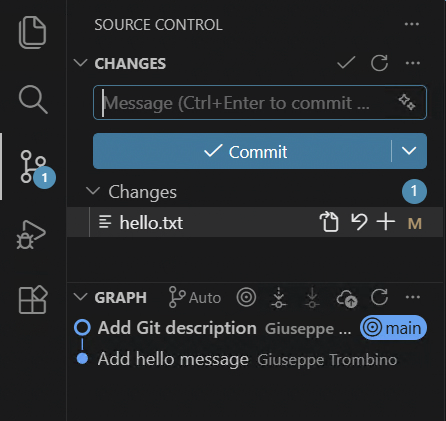
\includegraphics[width=0.85\textwidth]{../../../assets/figures/practical01/source control panel.png}
\label{fig:VSCodeSourceControlPanel}
\caption{The Visual Studio Code Source Control Panel}
\end{figure}
\subsection{Step 4: View the Changes}
Click:

\begin{terminalplain}
hello.txt
\end{terminalplain}
within the Source Control panel.

Visual Studio Code will display a comparison view showing:

\begin{itemize}
  \item The previous version of the file.
  \item The current version of the file.
\end{itemize}
Added lines are usually highlighted in green.

This is the graphical equivalent of:

\begin{terminalplain}
git diff
\end{terminalplain}
\subsection{Step 5: Stage the File Using the GUI}
In the Source Control panel, click the:

+

button beside:

\begin{terminalplain}
hello.txt
\end{terminalplain}
This stages the file.

In other words, VS Code has effectively performed:

\begin{terminalplain}
git add hello.txt
\end{terminalplain}
for you.

The computer did the typing this time.

\subsection{Step 6: Verify the Result}
Return to the terminal and run:

\begin{terminalplain}
git status
\end{terminalplain}
You should see something similar to:

\begin{terminalplain}
Changes to be committed:

\hspace*{1cm}\textcolor{GitGreen}{modified: hello.txt}
\end{terminalplain}
Notice that the terminal agrees with the graphical interface.

Both views are looking at the same repository.

\subsection{Step 7: Commit Using the GUI}
In the message box at the top of the Source Control panel, enter:

Add version control note

Click:

Commit

to create the commit.

\subsection{Step 8: Verify the Commit}
Return to the terminal and run:

\begin{terminalplain}
git log \mintinline{text}{--oneline}
\end{terminalplain}
You should now see three commits:

\begin{terminalplain}
  (HEAD -> main) Add version control note
  
  Add Git description
  
  Add hello message
\end{terminalplain}
  
Your commit identifiers will be different.

That is perfectly normal.

The important thing is that the new commit appears in the history.
\begin{reflectionbox}
  
  \textbf{What Just Happened?}\par
  \medskip
  You:
  
  \begin{itemize}
    \item Modified a file.
    \item Viewed the changes.
    \item Staged the changes.
    \item Created a commit.
  \end{itemize}
  Exactly the same workflow as Section 4.
  
  The only difference is that some of the commands were triggered by clicking buttons instead of typing them.
\end{reflectionbox}
  
\clearpage
\begin{importantnote}
  \textbf{A Note for the Future}\par
  \medskip
  Throughout the remainder of this module, examples will generally use Git commands in the terminal.
  
  This is because we will already be using the terminal to compile programs, run tests, and interact with repositories.
  
  However, you are welcome to use the VS Code interface whenever you find it convenient.
  
  Git does not particularly care how the commands were issued. Neither do I.
\end{importantnote}

\begin{reflectionbox}
\textbf{Checkpoint}\par
\medskip
Before continuing, confirm that you have:

Opened the Source Control panel.

Viewed a modified file.

Staged a file using the GUI.

Created a commit using the GUI.

Verified the commit using \mintinline{text}{git log --oneline}.
\end{reflectionbox}
\subsection{Common Problems}
\begin{commonerror}
\textbf{I Cannot See the Source Control Icon}\par
\medskip
Make sure that:
\end{commonerror}
\begin{itemize}
  \item The git-survival folder is open in VS Code.
  \item Git is installed correctly.
  \item You have initialised the repository using:
\end{itemize}
\begin{terminalplain}
git init
\end{terminalplain}
\begin{commonerror}
\textbf{The Commit Button Is Disabled}\par
\medskip
Ensure that:
\end{commonerror}
\begin{itemize}
  \item A commit message has been entered.
  \item The file has been staged.
\end{itemize}
\begin{commonerror}
\textbf{The File Does Not Appear in Source Control}\par
\medskip
Run:
\end{commonerror}
\begin{terminalplain}
git status
\end{terminalplain}
If Git does not report any changes, make sure the file has been saved.

This question continues to solve an alarming number of computing problems.

\begin{wrapupbox}
\textbf{Quest Complete}\par
\medskip
You have now used Git through both:

\begin{itemize}
  \item \faCheck\ The command line.
  \item \faCheck\ The Visual Studio Code graphical interface.
\end{itemize}

You now understand that both approaches operate on the same repository and perform the same underlying Git operations.

In the next section, you will learn how developers safely experiment with changes using branches.
\end{wrapupbox}

\section{Branching and Merging}
\begin{infobox}
\textbf{Estimated time: 15-20 minutes}
\end{infobox}
So far, every change you have made has been applied directly to the main version of your project.

In real software development, this is often not ideal.

What if you want to:

\begin{itemize}
  \item Try a new idea?
  \item Experiment with a feature?
  \item Make a change that might not work?
\end{itemize}
A branch allows you to work on changes without affecting the main version of the project.

Think of a branch as a safe place to experiment.

If things go well, you can merge the changes back into the main project.

If things go badly, the main project remains untouched.

\begin{learningoutcomes}
\textbf{What You Will Learn}\par
\medskip
By the end of this section, you should be able to:

\begin{itemize}
  \item Create a branch.
  \item Switch between branches.
  \item Observe how branches maintain separate versions of a project.
  \item Merge changes back into the main branch.
  \item Verify the result using Git history.
\end{itemize}
\textbf{A Tiny Bit of Theory}

A branch allows you to work on changes without immediately changing the main version of the project.

In this section, you will create a branch, make a change on that branch, observe that main has not changed yet, and then merge the branch back into main.

Don't worry too much about the details.

Let's see it in action.

\end{learningoutcomes}
\subsection{Step 1: View Existing Branches}
Run:

\begin{terminalplain}
git branch
\end{terminalplain}
You should see something similar to:

\begin{terminalplain}
  
  * main
\end{terminalplain}

The asterisk (*) indicates the branch you are currently using.

Most repositories start with a branch called \mintinline{text}{main}.

\subsection{Step 2: Create a New Branch}
Run:

\begin{terminalplain}
git branch feature-message
\end{terminalplain}
Nothing obvious will happen.

This is normal.

Git has created the branch, but you are still working on \mintinline{text}{main}.

\subsection{Step 3: Switch to the New Branch}
Run:

\begin{terminalplain}
git switch feature-message
\end{terminalplain}
You should see a message similar to:

\begin{terminalplain}
Switched to branch 'feature-message'
\end{terminalplain}
\subsection{Step 4: Verify Your Current Branch}
Run:

\begin{terminalplain}
git branch
\end{terminalplain}
You should now see:

\begin{terminalplain}
  
  * feature-message
  
  main

\end{terminalplain}

The asterisk has moved.

You are now working on \mintinline{text}{feature-message} instead of \mintinline{text}{main}.

\subsection{Step 5: Modify the File}
Open:

\begin{terminalplain}
hello.txt
\end{terminalplain}
Locate the line:

\begin{terminalplain}
Version control saves future headaches.
\end{terminalplain}
Replace it with:

\begin{terminalplain}
Version control saves future headaches and future tears.
\end{terminalplain}
Save the file.

\subsection{Step 6: Commit the Change}
Run:

\begin{terminalplain}
git add hello.txt
\end{terminalplain}
Then:

\begin{terminalplain}
git commit -m "Improve version control message"
\end{terminalplain}
You should see a message indicating that a new commit has been created.

\subsection{Step 7: View the History}
Run:

\begin{terminalplain}
git log \mintinline{text}{--oneline}
\end{terminalplain}
You should now see a new commit at the top of the history.

Your repository has continued to evolve on the \mintinline{text}{feature-message} branch.

\subsection{Step 8: Switch Back to Main}
Run:

\begin{terminalplain}
git switch main
\end{terminalplain}
You should see:

\begin{terminalplain}
Switched to branch 'main'
\end{terminalplain}
\subsection{Step 9: Open the File Again}
Open:

\begin{terminalplain}
hello.txt
\end{terminalplain}
Look carefully at the last line.

You should see:

\begin{terminalplain}
Version control saves future headaches.
\end{terminalplain}
The change has disappeared.

\begin{reflectionbox}
\textbf{What Has Happened?}\par
\end{reflectionbox}
\clearpage
Your project history now looks something like this:

\CSCGitBranchSplitDiagram

Where \textbf{A}, \textbf{B}, and \textbf{C} are the earlier commits, and \textbf{D} is a new commit created on \texttt{feature-message}.

Both branches share the first three commits. The new commit exists only on \texttt{feature-message}. That is why switching back to \texttt{main} makes the latest change disappear.

Git has not deleted anything. It is simply showing you the version of the project that belongs to the branch you selected.

\subsection{Step 10: Switch Back}
Run:

\begin{terminalplain}
git switch feature-message
\end{terminalplain}
Open:

\begin{terminalplain}
hello.txt
\end{terminalplain}
again.

The updated line should have returned:

\begin{terminalplain}
Version control saves future headaches and future tears.
\end{terminalplain}
Your work was never lost.

Git was simply showing you different versions of the project.

\begin{tipbox}
\textbf{A Small Observation}\par
\medskip
This is one of the main reasons developers use branches.

You can experiment freely without affecting the main version of the project. If your experiment works, you can merge it. If it does not, the main branch remains untouched.
\end{tipbox}

\subsection{Step 11: Merge the Branch}
Switch back to the main branch:

\begin{terminalplain}
git switch main
\end{terminalplain}
Then run:

\begin{terminalplain}
git merge feature-message
\end{terminalplain}
You should see a message similar to:

\begin{terminalplain}
Updating \ldots{}

Fast-forward
\end{terminalplain}
The merge has completed successfully.

\subsection{Step 12: Verify the Result}
Open:

\begin{terminalplain}
hello.txt
\end{terminalplain}
You should now see:

\begin{terminalplain}
Version control saves future headaches and future tears.
\end{terminalplain}
The change now exists on \texttt{main} as well.

\CSCGitFastForwardDiagram

\subsection{Step 13: View the History}
Run:

\begin{terminalplain}
git log \mintinline{text}{--oneline}
\end{terminalplain}
You should see all of your previous commits, including:

Improve version control message

The branch and the main project now contain the same work.

\begin{reflectionbox}
\textbf{Checkpoint}\par
\medskip
Before continuing, confirm that you have:

Created a branch.

Switched between branches.

Observed different versions of the project.

Created a commit on a branch.

Successfully merged the branch.

Verified the merge using \mintinline{text}{git log --oneline}.
\end{reflectionbox}
\subsection{Common Problems}
\begin{commonerror}
\textbf{"fatal: invalid reference"}\par
\medskip
Check the branch name carefully.

Git branch names must match exactly.

Run:

\begin{terminalplain}
  git branch
\end{terminalplain}
to see the available branches.
\end{commonerror}

\begin{commonerror}
\textbf{My Changes Have Disappeared}\par
\medskip
They probably haven't.

Run:

\begin{terminalplain}
  git branch
\end{terminalplain}
to see which branch you are currently using.

Then switch back if necessary:

\begin{terminalplain}
  git switch feature-message
\end{terminalplain}
\end{commonerror}
\begin{commonerror}
\textbf{Git Says There Is Nothing to Merge}\par
\medskip
You may already be on the latest version.

Run:

\begin{terminalplain}
  git log \mintinline{text}{--oneline}
\end{terminalplain}
and compare your commit history.
\end{commonerror}

\begin{wrapupbox}
\textbf{Quest Complete}\par
\medskip
You have now:

\begin{itemize}
  \item \faCheck\ Created a branch.
  \item \faCheck\ Worked on an isolated version of a project.
  \item \faCheck\ Switched between branches.
  \item \faCheck\ Merged changes back into the main project.
\end{itemize}

This is one of the most common workflows used in professional software development.

In the next section, we will deliberately create a merge conflict and learn how to resolve it safely.

For the first time in this lab, things will \textbf{NOT} go entirely according to plan.
\end{wrapupbox}

\section{Resolving Merge Conflicts}
\begin{infobox}
\textbf{Estimated time: 15-20 minutes}
\end{infobox}
In the previous section, Git merged two branches automatically.

Everything worked exactly as expected.

However, there are situations where Git cannot safely decide how two changes should be combined.

When this happens, Git stops and asks for help.

This situation is known as a \textbf{merge conflict}.

A merge conflict does \textbf{NOT} mean that Git is broken.

It simply means that Git needs you to make a decision.

In this section, we will deliberately create a merge conflict and then resolve it.

\begin{learningoutcomes}
\textbf{What You Will Learn}\par
\medskip
By the end of this section, you should be able to:

\begin{itemize}
  \item Understand why merge conflicts occur.
  \item Recognise a merge conflict.
  \item Identify the conflicting changes.
  \item Resolve a merge conflict manually.
  \item Complete a merge after resolving a conflict.
\end{itemize}
\end{learningoutcomes}
\subsection{Step 1: Create a New Branch}
Run:

\begin{terminalplain}
git switch -c feature-warning
\end{terminalplain}
You should see a message similar to:

\begin{terminalplain}
Switched to a new branch 'feature-warning'
\end{terminalplain}
\subsection{Step 2: Modify the File}
Open:

\begin{terminalplain}
hello.txt
\end{terminalplain}
Locate the line:

\begin{terminalplain}
Version control saves future headaches and future tears.
\end{terminalplain}
Replace it with:

\begin{terminalplain}
Version control saves future headaches, future tears, and future panic.
\end{terminalplain}
Save the file.

\subsection{Step 3: Commit the Change}
Run:

\begin{terminalplain}
git add hello.txt
\end{terminalplain}
Then:

\begin{terminalplain}
git commit -m "Add panic warning"
\end{terminalplain}
\subsection{Step 4: Return to Main}
Run:

\begin{terminalplain}
git switch main
\end{terminalplain}
You should see:

\begin{terminalplain}
Switched to branch 'main'
\end{terminalplain}
\subsection{Step 5: Make a Different Change}
Open:

\begin{terminalplain}
hello.txt
\end{terminalplain}
again.

Locate the same line:

\begin{terminalplain}
Version control saves future headaches and future tears.
\end{terminalplain}
Replace it with:

\begin{terminalplain}
Version control saves future headaches, future tears, and future confusion.
\end{terminalplain}
Save the file.

\subsection{Step 6: Commit the Change}
Run:

\begin{terminalplain}
git add hello.txt
\end{terminalplain}
Then:

\begin{terminalplain}
git commit -m "Add confusion warning"
\end{terminalplain}
\begin{reflectionbox}
\textbf{What Has Happened?}\par
\medskip
At this point:

\begin{itemize}
  \item The main branch contains the word \textbf{confusion}.
  \item The feature-warning branch contains the word \textbf{panic}.
\end{itemize}
Both branches changed the same line.
\end{reflectionbox}

The project history now looks something like this:

\CSCGitConflictDiagram

The two branches now disagree.

\begin{reflectionbox}
\textbf{Think Before You Type}\par
\medskip
If Git tries to merge these branches, what should it do?

Should it keep:
\begin{itemize}
  \item \texttt{panic}?
  \item \texttt{confusion}?
  \item both?
\end{itemize}
Git does not know the answer. Let's see what happens.
\end{reflectionbox}

\subsection{Step 7: Attempt the Merge}
Run:

\begin{terminalplain}
git merge feature-warning
\end{terminalplain}
You should see something similar to:

\begin{terminalplain}
CONFLICT (content): Merge conflict in hello.txt
\end{terminalplain}
\begin{terminalplain}
Automatic merge failed
\end{terminalplain}
\begin{importantnote}
\textbf{Good!}\par
\medskip
This is exactly what we wanted.

For the first time in this lab, Git has encountered a situation that it cannot resolve automatically.

Rather than guessing, Git has stopped and asked for help.
\end{importantnote}
\subsection{Step 8: Open the File}
Open:

\begin{terminalplain}
hello.txt
\end{terminalplain}
You should now see something similar to:

\begin{minted}{text}
<<<<<<< HEAD
Version control saves future headaches, future tears, and future confusion.
=======
Version control saves future headaches, future tears, and future panic.
>>>>>>> feature-warning
\end{minted}

\begin{importantnote}
\textbf{Understanding the Markers}\par
\medskip
The line \mintinline{text}{<<<<<<< HEAD} marks the version currently on \texttt{main}. The line \texttt{=======} separates the two versions. The line \mintinline{text}{>>>>>>> feature-warning} marks the version coming from the \texttt{feature-warning} branch.

These markers were added by Git to identify the conflicting versions. They must be removed before the merge can be completed.
\end{importantnote}

\subsection{Step 9: Resolve the Conflict}
Replace the entire conflict block with:

\begin{quote}
\mintinline{text}{Version control saves future headaches, future tears, future confusion, and future panic.}
\end{quote}
Your file should no longer contain the conflict markers \mintinline{text}{<<<<<<<}, \mintinline{text}{=======}, or \mintinline{text}{>>>>>>>}.

Save the file.

\subsection{Step 10: Stage the Resolved File}
Run:

\begin{terminalplain}
git add hello.txt
\end{terminalplain}
\subsection{Step 11: Complete the Merge}
Run:

\begin{terminalplain}
git commit -m "Resolve merge conflict"
\end{terminalplain}
The merge is now complete.
\begin{importantnote}
\textbf{Advanced Note}\par
\medskip
Modern versions of Git also support:

\begin{terminalplain}
  git merge \mintinline{text}{--continue}
\end{terminalplain}
which completes an in-progress merge after conflicts have been resolved (or moves to the next unresolved conflict).

For this lab, we will continue using git commit -m \ldots{} because it follows the workflow you have already learned.
\end{importantnote}

\subsection{Step 12: Verify the Result}
Run:

\begin{terminalplain}
git log \mintinline{text}{--oneline}
\end{terminalplain}
You should see a new commit similar to \texttt{Resolve merge conflict} near the top of the history.

\CSCGitConflictResolvedDiagram

\begin{reflectionbox}
\textbf{What Just Happened?}\par
\medskip
Let's review:

\begin{enumerate}
  \item Two branches modified the same line.
  \item Git could not determine which version should be kept.
  \item Git asked you to decide.
  \item You resolved the conflict manually.
  \item The merge completed successfully.
\end{enumerate}
At no point was any work lost.

Git simply refused to guess.
\end{reflectionbox}

\begin{reflectionbox}
\textbf{Checkpoint}\par
\medskip
Before continuing, confirm that you have:

Created a merge conflict.

Opened the conflicted file.

Identified the conflict markers.

Resolved the conflict manually.

Completed the merge.

Verified the result using \mintinline{text}{git log --oneline}.
\end{reflectionbox}
\subsection{Common Problems}
\begin{commonerror}
\textbf{Git Says "You Have Unmerged Paths"}\par
\medskip
Good.

You are probably in the middle of the exercise.

Resolve the conflict in the file first, then run:

\begin{terminalplain}
  git add hello.txt
\end{terminalplain}
before attempting to commit.
\end{commonerror}

\begin{commonerror}
\textbf{The Strange Markers Are Still Visible}\par
\medskip
Ensure that all of the following lines have been removed:

\begin{terminalplain}
  \mintinline{text}{<<<<<<<}

  =======
  
  \mintinline{text}{>>>>>>>}
\end{terminalplain}

Git cannot complete the merge while these markers remain in the file.
\end{commonerror}

\begin{commonerror}
\textbf{I Accidentally Deleted Everything}\par
\medskip
Do not panic.

Git repositories are surprisingly difficult to damage permanently.

Ask a demonstrator for assistance.
\end{commonerror}
\begin{wrapupbox}
\textbf{Quest Complete}\par
\medskip
You have now:

\begin{itemize}
  \item \faCheck\ Created a merge conflict.
  \item \faCheck\ Understood why the conflict occurred.
  \item \faCheck\ Resolved the conflict manually.
  \item \faCheck\ Completed the merge successfully.
\end{itemize}

Most importantly:

\begin{itemize}
  \item \faCheck\ Learned that merge conflicts are a normal part of software development.
\end{itemize}

In the next section, we will connect Git to GitHub and prepare for using Classroom50 repositories.
\end{wrapupbox}

\section{Preparing Your GitHub Account}
\begin{infobox}
\textbf{Estimated time: 10-15 minutes}
\end{infobox}
Throughout this module, you will access repositories and submit work using GitHub-based tools.

Before we can do that, we need to make sure that your GitHub account is correctly configured.

In particular, your university email address should be associated with your GitHub account.

This will help ensure that repositories, coursework, and classroom activities can be linked to the correct student account.

\begin{learningoutcomes}
\textbf{What You Will Learn}\par
\medskip
By the end of this section, you should be able to:

\begin{itemize}
  \item Create a GitHub account (if necessary).
  \item Log into GitHub.
  \item Add your university email address to your GitHub account.
  \item Verify your university email address.
  \item Confirm that your account is ready for use in CSC2059.
\end{itemize}
\end{learningoutcomes}
\subsection{Before You Begin}
If you already have a GitHub account:

\textbf{Do not create a second account.}

GitHub allows multiple email addresses to be associated with a single account.

Most professional developers use a single GitHub account throughout their careers, even when they change employers or educational institutions.

If you already have an account, simply add your university email address to it.

\subsection{Step 1: Sign In/Sign Up to GitHub}
Open your web browser and visit:

\url{https://github.com}

Sign in using your existing account.

If you do not already have a GitHub account, create one now.

\begin{reflectionbox}
\textbf{Checkpoint}\par
\medskip
Before continuing, confirm that:

You can successfully sign in to GitHub.
\end{reflectionbox}
\subsection{Step 2: Open Your Account Settings}
Click your profile picture in the top-right corner of GitHub.

Select:

Settings

from the menu.

\subsection{Step 3: Open Email Settings}
In the left-hand navigation menu, locate:

Emails

and select it. (See Figure~\ref{fig:AddGitHubEmail})

\subsection{Step 4: Add Your University Email Address}
Locate the option to add an email address.

Enter your university email address.

For example:

jsmith123@qub.ac.uk

Use your own university email address, not the example above.

Submit the change.

\begin{figure}[htbp]
\centering
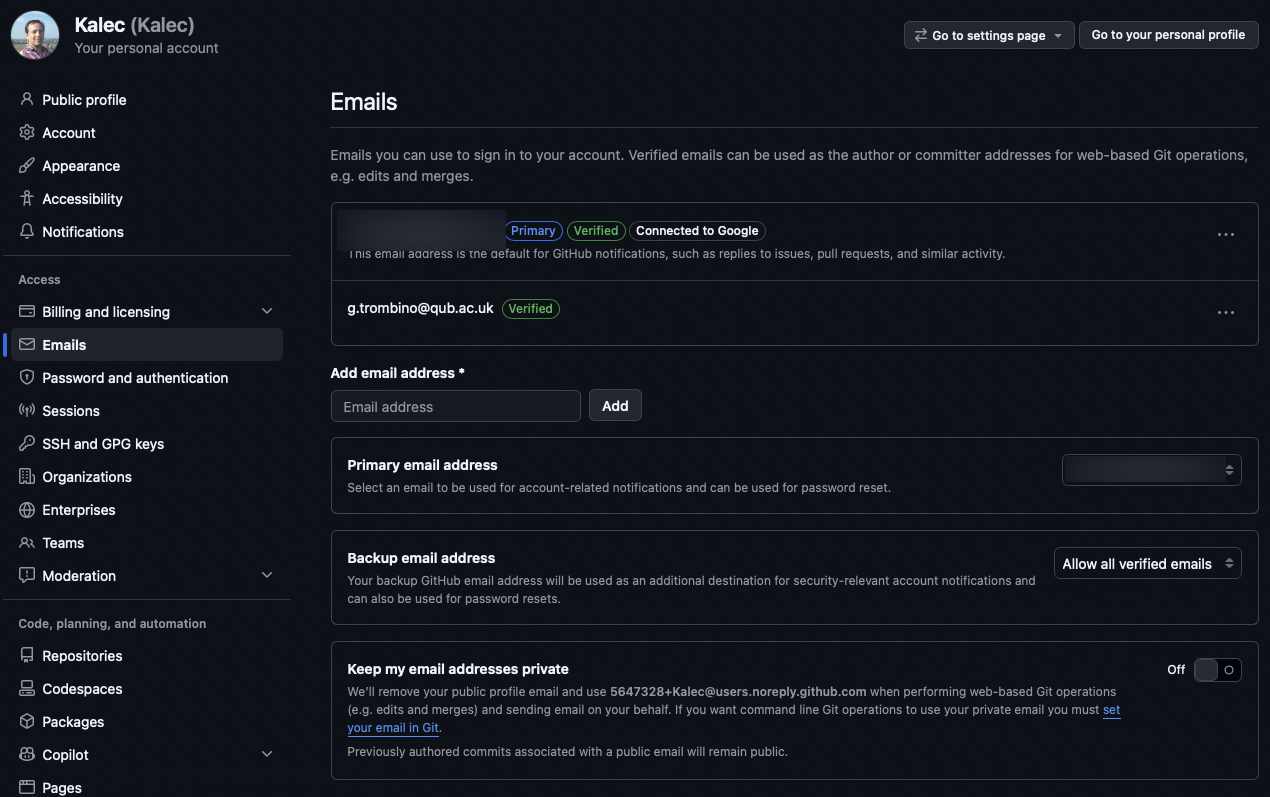
\includegraphics[width=0.9\textwidth]{../../../assets/figures/practical01/AddGitHubEmail.png}
\caption{GitHub Email Settings Page}
\label{fig:AddGitHubEmail}
\end{figure}
\subsection{Step 5: Verify Your Email Address}
GitHub will send a verification email to the address you provided.

Open your university email account.

Locate the GitHub verification email.

Follow the verification instructions provided by GitHub.

\subsection{Step 6: Confirm Verification}
Return to GitHub.

Refresh the Email Settings page if necessary.

Your university email address should now appear as:

Verified

or equivalent.
\begin{importantnote}
\textbf{Why Are We Doing This?}\par
\medskip
Later in this module, you will access repositories through GitHub-based classroom systems.

Having a verified university email address associated with your account helps ensure that:

\begin{itemize}
  \item Your account can be identified correctly.
  \item Repository access can be granted more easily.
  \item Coursework repositories are associated with the correct student.
\end{itemize}
Spending a few minutes on this now can save a considerable amount of troubleshooting later.
\end{importantnote}

\begin{reflectionbox}
\textbf{Checkpoint}\par
\medskip
Before continuing, confirm that:

You can log into GitHub.

Your university email address has been added.

Your university email address has been verified.
\end{reflectionbox}
\subsection{Common Problems}
\begin{commonerror}
\textbf{I Already Have a GitHub Account}\par
\medskip
Excellent.

Use your existing account.

Simply add your university email address and verify it.
\end{commonerror}
\begin{commonerror}
\textbf{I Cannot Find the Verification Email}\par
\medskip
Check:

\begin{itemize}
  \item Your inbox.
  \item Your junk/spam folder.
  \item Any filtered folders used by your email system.
\end{itemize}
If necessary, request that GitHub resend the verification email.
\end{commonerror}

\begin{commonerror}
\textbf{I Added the Email but It Still Shows as Unverified}\par
\medskip
Verification emails occasionally take a few minutes to arrive.

Wait a short time and refresh the page.

If the problem persists, ask a demonstrator for assistance.
\end{commonerror}
\begin{wrapupbox}
\textbf{Quest Complete}\par
\medskip
You have now:

\begin{itemize}
  \item \faCheck\ Logged into GitHub.
  \item \faCheck\ Associated your university email address with your account.
  \item \faCheck\ Verified your university email address.
  \item \faCheck\ Prepared your account for use in CSC2059.
\end{itemize}

You now possess the core Git skills needed for this module:

\begin{itemize}
  \item Creating repositories
  \item Tracking changes
  \item Creating commits
  \item Working with branches
  \item Resolving merge conflicts
  \item Using GitHub
\end{itemize}

In future labs, you will connect these skills to coursework repositories and automated testing workflows.
\end{wrapupbox}
\section{Further Practice (Optional)}
The activities in this lab are sufficient preparation for CSC2059.

However, like any practical skill, confidence comes from practice.

If you would like additional opportunities to explore Git, the following resources are recommended. These are entirely optional, but many students find them useful for reinforcing the concepts introduced in this lab.

\subsection{Interactive Git Tutorial}
\subsubsection{Learn Git Branching}
\url{https://learngitbranching.js.org}

This is one of the most popular Git learning tools available online.

It provides an interactive environment where you can experiment with:

\begin{itemize}
  \item Branching
  \item Merging
  \item Rebasing
  \item Remote repositories
\end{itemize}
without affecting any real repositories.

The visual approach is particularly useful for understanding how branches and commits are related.

\textbf{Recommended after:} Sections 6 and 7 (Branching and Merge Conflicts).

\subsection{Guided Git Tutorial}
\subsubsection{W3Schools Git Tutorial}
\url{https://www.w3schools.com/git/}

This tutorial provides a structured introduction to Git concepts and commands.

It covers many of the topics introduced in this lab, including:

\begin{itemize}
  \item Repositories
  \item Commits
  \item Branches
  \item Merging
  \item Remote repositories
\end{itemize}
It can be useful as a reference if you would like additional examples or explanations.

\textbf{Recommended after:} Completing this lab.

\begin{importantnote}
\textbf{A Small Warning}\par
\medskip
It is easy to fall into the trap of spending hours reading about Git without actually using it.

The best way to learn Git is to:

\begin{enumerate}
  \item Create repositories.
  \item Make changes.
  \item Create commits.
  \item Break things occasionally.
  \item Fix them.
\end{enumerate}

In other words, \textbf{use Git}.

The coursework, laboratory exercises, and programming tasks throughout CSC2059 will provide plenty of opportunities to do exactly that.
\end{importantnote}
\section{Challenge Quest}
If you would like an extra challenge, try creating a brand-new repository and reproduce the following workflow without referring to this guide:
\VerticalWorkflowSeven
  {Create Repository}
  {Create File}
  {Commit}
  {Create Branch}
  {Modify File}
  {Commit}
  {Merge Branch}

If you can complete that sequence successfully, you are well on your way to becoming comfortable with Git.

Good luck, and remember:

\begin{terminalplain}
git status
\end{terminalplain}
solves a surprising number of Git-related mysteries.

\section{Git Best Practices}
Throughout this module, Git will be used to track your development work.

Like any tool, Git works best when used consistently.

The following habits will save you time, reduce stress, and make it easier to recover from mistakes.

\subsection{Commit Early, Commit Often}
One of the most common mistakes made by new Git users is waiting until the very end of a task before creating a commit.

Instead, try to create commits whenever you complete a small, meaningful piece of work.

For example:

\begin{itemize}
  \item \faCheck\ Good:
\end{itemize}
Create class

↓

Commit

Implement constructor

↓

Commit

Implement search function

↓

Commit

Fix failing test

↓

Commit

\begin{itemize}
  \item \faTimes\ Less helpful:
\end{itemize}
Work for three hours

↓

Commit everything

Smaller commits make it much easier to:

\begin{itemize}
  \item Recover from mistakes.
  \item Understand what changed.
  \item Identify when a problem was introduced.
  \item Return to an earlier working version.
\end{itemize}
\subsection{Write Meaningful Commit Messages}
A commit message should briefly describe \textbf{what changed}.

Good commit messages help both you and others understand the history of a project.

\subsubsection{Examples of Good Commit Messages}
\begin{quote}
  Add search function
  
  Fix off-by-one error in loop
  
  Implement Stack::push()
  
  Resolve merge conflict
  
  Add unit tests for linked list
\end{quote}

These messages clearly describe the change that was made.

\subsubsection{Examples of Less Helpful Commit Messages}

\begin{quote}
  Stuff
  
  Update
  
  Work in progress / WIP
  
  Changes
  
  asdf
\end{quote}

While Git will happily accept these messages, they provide very little useful information.

Six weeks later, even the person who wrote them may have no idea what they mean.

\subsection{Commit Working Code When Possible}
A useful rule of thumb is:

If the code compiles and passes the tests, it is probably a good time to commit.

This does not mean every commit must be perfect.

However, creating commits at logical milestones makes your repository history easier to understand and use.

\subsection{Check Before You Commit}
Before creating a commit, it is often worth running:

\begin{terminalplain}
git status
\end{terminalplain}
and, if appropriate:

\begin{terminalplain}
git diff
\end{terminalplain}
These commands allow you to confirm exactly what is about to be included in the commit.

A few seconds spent checking can prevent a lot of confusion later.

\subsection{Push Regularly}
Later in this module, you will work with remote repositories.

When that happens, remember:

A commit only exists on your computer until it is pushed.

\CSCGitRemoteDiagram
Creating commits regularly is good.

Creating commits and pushing them regularly is even better.

Computers occasionally fail.

Repositories stored remotely are much harder to lose.

\subsection{A Habit Worth Developing}
Many experienced developers follow a simple cycle:
\begin{center}
  Make a small change
  
  ↓
  
  Test it
  
  ↓
  
  Commit it
  
  ↓
  
  Repeat
\end{center}

It may feel slow at first.

In practice, it is usually much faster than trying to recover from several hours of lost work.

\subsection{Final Thought}
Git is most useful when it becomes part of your normal workflow rather than something you remember to use at the last minute.

Future-you will be very grateful to present-you for creating clear commit messages and regular commits.

Trust us on this one.

\section{Lab Summary}
Congratulations.

You have completed the first CSC2059 laboratory exercise.

When you started this lab, Git may have been completely unfamiliar. By this point, you have successfully used many of the core tools and workflows that software developers use every day.

During this lab, you have learned how to:

\begin{itemize}
  \item \faCheck\ Configure Git for use in CSC2059.
  \item \faCheck\ Create and manage Git repositories.
  \item \faCheck\ Track changes to files.
  \item \faCheck\ Stage and commit changes.
  \item \faCheck\ Review repository history.
  \item \faCheck\ Use both the command line and the Visual Studio Code interface.
  \item \faCheck\ Create and switch between branches.
  \item \faCheck\ Merge changes safely.
  \item \faCheck\ Resolve merge conflicts.
  \item \faCheck\ Configure a GitHub account for use in this module.
\end{itemize}
You have also encountered an important lesson:

Git is not a magic box.

It is a tool that records changes, helps you organise your work, and occasionally asks sensible questions when it is unsure what you want.

Throughout the rest of CSC2059, you will use Git regularly to:

\begin{itemize}
  \item Access laboratory exercises.
  \item Access coursework repositories.
  \item Track your development progress.
  \item Submit work.
  \item Collaborate with automated testing systems.
\end{itemize}
The commands introduced in this lab will appear again and again throughout the module.

In particular, you should become comfortable using:

\begin{terminalplain}
git status
git add
git commit
git log
git branch
git switch
git merge
\end{terminalplain}
If you forget how any of these commands work, return to this guide and use it as a reference.

Nobody memorises everything the first time.

The goal of this lab was not to turn you into a Git expert.

The goal was to give you the skills needed to work confidently and safely throughout the rest of the module.

Mission accomplished.

See you in Lab 2.

\end{document}
